\documentclass[11pt]{article}
\usepackage[T1]{fontenc}
\usepackage{lmodern}
\usepackage[a4paper,margin=2cm]{geometry}
\usepackage{xcolor}
\usepackage{siunitx}
\usepackage{booktabs}
\usepackage{array}
\usepackage{tikz}
\usepackage{pgfplots}
\pgfplotsset{compat=1.18}
\usepackage{enumitem}
\usepackage{amsmath,amssymb}

\renewcommand{\familydefault}{\sfdefault}
\pagestyle{empty}
\setlength{\parindent}{0pt}
\setlength{\parskip}{0.4em}
\definecolor{labhead}{RGB}{0,105,92}
\definecolor{fillbg}{RGB}{240,247,246}

% A blank line to write on: \blank{width}
\newcommand{\blank}[1]{\underline{\hspace{#1}}}

% Numbered worksheet step with a coloured tab.
\newcounter{step}
\newcommand{\step}[1]{\par\bigskip\refstepcounter{step}%
  \colorbox{labhead}{\color{white}\bfseries\ \thestep\ }\hspace{0.5em}{\large\bfseries\color{labhead}#1}\par\smallskip}

\begin{document}

% Worksheet title and student fields.
{\color{labhead}\rule{\textwidth}{2pt}}\par
{\LARGE\bfseries Lab 5: Hooke's Law and Spring Constants}\hfill{\small Physics 101}\par
{\color{labhead}\rule{\textwidth}{0.6pt}}

\begin{tabular}{@{}l p{5.5cm} l p{4.5cm}@{}}
  Name: & Sky Bennett & Date: & \today \\
  Lab partner: & Drew Palmer & Group: & B3 \\
\end{tabular}

\step{Aim}
To measure the extension of a spring under different loads and determine its spring constant $k$ using $F = kx$.

\step{Equipment}
\begin{itemize}[leftmargin=1.5em,itemsep=0pt]
  \item Spring, retort stand and clamp
  \item Slotted masses (\SI{50}{\gram} each) on a hanger
  \item Metre rule with \SI{1}{\milli\metre} resolution
\end{itemize}

\step{Safety check}
% Tick the boxes before starting.
$\square$ Stand clamped to the bench \qquad $\square$ Goggles worn \qquad $\square$ Masses kept below \SI{500}{\gram}

\step{Results}
Record the extension for each load. Take $g = \SI{9.81}{\metre\per\second\squared}$.

\begin{center}
\renewcommand{\arraystretch}{1.3}
\begin{tabular}{S[table-format=3.0] S[table-format=1.3] S[table-format=2.1] S[table-format=2.1] S[table-format=2.1]}
  \toprule
  {Mass (\si{\gram})} & {Force (\si{\newton})} & {Trial 1 (\si{\milli\metre})} & {Trial 2 (\si{\milli\metre})} & {Mean $x$ (\si{\milli\metre})} \\
  \midrule
  50  & 0.491 & 12.0 & 12.4 & 12.2 \\
  100 & 0.981 & 24.5 & 24.1 & 24.3 \\
  150 & 1.472 & 36.2 & 36.8 & 36.5 \\
  200 & 1.962 & 48.9 & 48.3 & 48.6 \\
  250 & 2.453 & 60.7 & 61.1 & 60.9 \\
  \bottomrule
\end{tabular}
\end{center}

\step{Graph}
Plot force against mean extension and draw a line of best fit.

\begin{center}
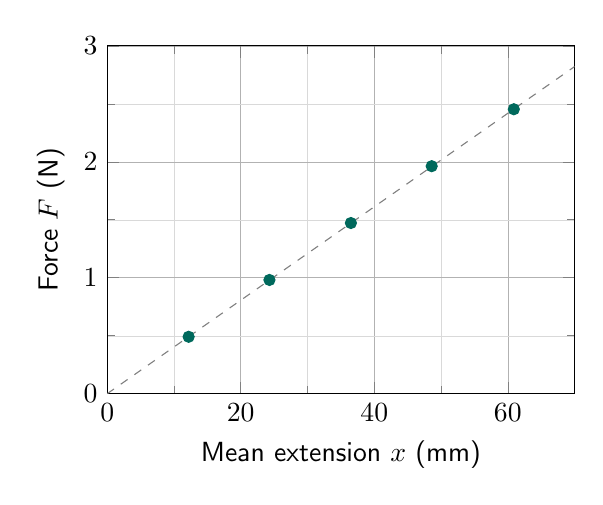
\begin{tikzpicture}
  \begin{axis}[
    width=0.62\textwidth, height=6cm,
    xlabel={Mean extension $x$ (mm)}, ylabel={Force $F$ (N)},
    xmin=0, xmax=70, ymin=0, ymax=3,
    grid=both, minor tick num=1,
    grid style={line width=0.1pt,draw=gray!30},
    major grid style={line width=0.2pt,draw=gray!60}]
    % Replace these points with your own measurements.
    \addplot[only marks,mark=*,labhead] coordinates {(12.2,0.491) (24.3,0.981) (36.5,1.472) (48.6,1.962) (60.9,2.453)};
    \addplot[samples=2,domain=0:70,dashed,gray] {0.0403*x};
  \end{axis}
\end{tikzpicture}
\end{center}

\step{Analysis}
\colorbox{fillbg}{\begin{minipage}{\dimexpr\textwidth-2\fboxsep}
  Gradient of the line: $\dfrac{\Delta F}{\Delta x} = $ \blank{3cm} \si{\newton\per\milli\metre}\par\medskip
  Spring constant: $k = $ \blank{3cm} \si{\newton\per\metre}\par\medskip
  Percentage difference from the value on the spring label (\SI{40}{\newton\per\metre}): \blank{2.5cm} \%
\end{minipage}}

\step{Questions}
\begin{enumerate}[label=\alph*),leftmargin=2em]
  \item Does your graph pass through the origin? What would it mean if it did not?\par
        \blank{\linewidth}\par\blank{\linewidth}
  \item Name one source of random error and one of systematic error in this experiment.\par
        \blank{\linewidth}\par\blank{\linewidth}
\end{enumerate}

\step{Conclusion}
\fbox{\begin{minipage}[t][2.2cm][t]{\dimexpr\textwidth-2\fboxsep-2\fboxrule}\color{gray}\small Summarise your result for $k$ and how confident you are in it.\end{minipage}}

\end{document}
